\chapter{Experimental Results}
\label{ch:results}

All numbers in this chapter are generated by \texttt{scripts/analyze.py} and
\texttt{scripts/make\_numbers.py} from the run directories, so they cannot drift
from the logs. Means and standard deviations are over the seeds stated in each
table. The test sets were evaluated once per run, with the checkpoint chosen on
validation data.

\section{Main comparison}
\begin{table}[h]
\centering
\caption{RadHAR official test recordings (3{,}565 windows, 5 classes). Mean\,$\pm$\,std over 3 seeds. Sig.: number of seeds in which the Holm-corrected McNemar test against the proposed model gives $p<0.05$; $\uparrow$ ours better / $\downarrow$ ours worse. Latency: median, batch 1, one CPU thread.}
\label{tab:radharreport}
\setlength{\tabcolsep}{5pt}
\resizebox{\textwidth}{!}{\begin{tabular}{lrrrccc}
\toprule
Model & Params (K) & MFLOPs & Lat. (ms) & Accuracy (\%) & Macro-F1 (\%) & Sig. \\
\midrule
Voxel TD-CNN+BiLSTM [RadHAR] & 45.9 & 180.5 & 6.60 & 95.01\,$\pm$\,0.16 & 95.03\,$\pm$\,0.17 & 2/3$\uparrow$ \\
PointNet & 76.2 & 31.8 & 0.74 & 96.31\,$\pm$\,0.66 & 96.36\,$\pm$\,0.64 & 1/3$\uparrow$ \\
PointNet+BiLSTM & 109.1 & 6.6 & 0.83 & 96.14\,$\pm$\,0.23 & 96.16\,$\pm$\,0.21 & 2/3$\uparrow$ \\
PointNet++ (SSG) & 413.4 & 133.1 & 8.44 & 97.34\,$\pm$\,0.18 & 97.37\,$\pm$\,0.19 & 1/3$\downarrow$ \\
DGCNN & 422.4 & 137.9 & 6.95 & 95.85\,$\pm$\,0.00 & 95.89\,$\pm$\,0.00 & 1/3$\uparrow$ \\
Point Transformer & 335.2 & 264.4 & 7.98 & 97.01\,$\pm$\,0.25 & 97.04\,$\pm$\,0.24 & 1/3$\uparrow$ \\
\midrule
STPT-Large (teacher) & 725.3 & 139.5 & 3.59 & 96.44\,$\pm$\,1.43 & 96.48\,$\pm$\,1.42 & 1/3$\uparrow$ \\
STPT-Lite & 117.5 & 36.6 & 2.14 & 96.22\,$\pm$\,1.43 & 96.27\,$\pm$\,1.41 & 2/3$\uparrow$ \\
STPT-Lite + KD & 117.5 & 36.6 & 2.08 & 96.04\,$\pm$\,0.78 & 96.08\,$\pm$\,0.76 & 1/3$\uparrow$ \\
STPT-Tiny + KD & 30.7 & 12.1 & 1.92 & 96.86\,$\pm$\,0.17 & 96.90\,$\pm$\,0.16 & 1/3$\uparrow$ \\
\textbf{STPT-Lite + KD + robust (ours)} & 117.5 & 36.6 & 2.58 & 96.83\,$\pm$\,0.69 & 96.88\,$\pm$\,0.68 & -- \\
PointNet + noise-robust training & 76.2 & 31.8 & 0.73 & \textbf{97.38\,$\pm$\,0.11} & \textbf{97.40\,$\pm$\,0.11} & 1/3$\downarrow$ \\
\bottomrule
\end{tabular}}
\end{table}
\begin{table}[h]
\centering
\caption{MiliPoint, subject-disjoint test (subjects 8--10, 3{,}569 windows, 49 actions). Same conventions as Table~\ref{tab:radharreport}.}
\label{tab:mpreport}
\setlength{\tabcolsep}{5pt}
\resizebox{\textwidth}{!}{\begin{tabular}{lrrrccrc}
\toprule
Model & Params (K) & MFLOPs & Lat. (ms) & Accuracy (\%) & Macro-F1 (\%) & Top-3 & Sig. \\
\midrule
PointNet & 81.9 & 31.8 & 0.74 & 32.57\,$\pm$\,4.59 & 29.72\,$\pm$\,4.50 & 59.5 & 3/3$\uparrow$ \\
PointNet+BiLSTM & 114.8 & 6.6 & 0.74 & 28.11\,$\pm$\,4.06 & 28.09\,$\pm$\,4.66 & 56.1 & 3/3$\uparrow$ \\
PointNet++ (SSG) & 424.7 & 133.1 & 7.94 & 8.07\,$\pm$\,5.47 & 5.12\,$\pm$\,5.76 & 21.4 & 3/3$\uparrow$ \\
STPT-Large (teacher) & 730.9 & 139.5 & 3.65 & \textbf{50.39\,$\pm$\,1.39} & \textbf{50.84\,$\pm$\,2.11} & 75.8 & 1/3$\uparrow$ \\
STPT-Lite & 120.4 & 36.6 & 2.60 & 45.79\,$\pm$\,6.30 & 45.95\,$\pm$\,7.05 & 73.9 & 1/3$\uparrow$ \\
STPT-Lite + KD & 120.4 & 36.6 & 2.07 & 48.55\,$\pm$\,4.35 & 47.62\,$\pm$\,6.08 & 76.4 & 1/3$\downarrow$ \\
\textbf{STPT-Lite + KD + robust (ours)} & 120.4 & 36.6 & 2.00 & 49.56\,$\pm$\,1.98 & 48.80\,$\pm$\,1.68 & 78.0 & -- \\
PointNet + noise-robust training & 81.9 & 31.8 & 0.78 & 18.66\,$\pm$\,8.83 & 15.67\,$\pm$\,8.98 & 40.9 & 3/3$\uparrow$ \\
\bottomrule
\end{tabular}}
\end{table}

\textbf{MiliPoint, unseen subjects (Table~\ref{tab:mpreport}).} The
STPT family clearly outperforms all re-implemented baselines.
The proposed STPT-Lite+KD+robust (selected on validation macro-F1, Issue~\#39)
reaches \mistptlitekdrobustAcc\,$\pm$\,\mistptlitekdrobustStd\% top-1
(\mistptlitekdrobustTopthree\% top-3); distillation alone gives
\mistptlitekdAcc\,$\pm$\,\mistptlitekdStd\%. This compares with \mipointnetAcc\,$\pm$\,\mipointnetStd\% for
the best baseline (PointNet). Every pairwise difference to a baseline is
significant in all three seeds (exact McNemar, Holm-corrected, $p<10^{-45}$).
Distillation raised the mean and, above all, removed a failed seed (STPT-Lite
without KD: one seed at 38.6\%).

\textbf{RadHAR (Table~\ref{tab:radharreport}).} All point-based models lie
between about 96 and 98\%, and differences between them are mostly within one
standard deviation. The proposed model reaches \rastptlitekdrobustAcc\,$\pm$\,\rastptlitekdrobustStd\%.
PointNet++ is the most accurate here, at 4--5$\times$ our
latency and 3.5$\times$ our parameter count. Every model, including the voxel
CNN-LSTM from the original paper, exceeds the published 90.47\%, which shows
the effect of the shared pre-processing.

\section{Per-class results and confusion}
\begin{figure}[h]
\centering
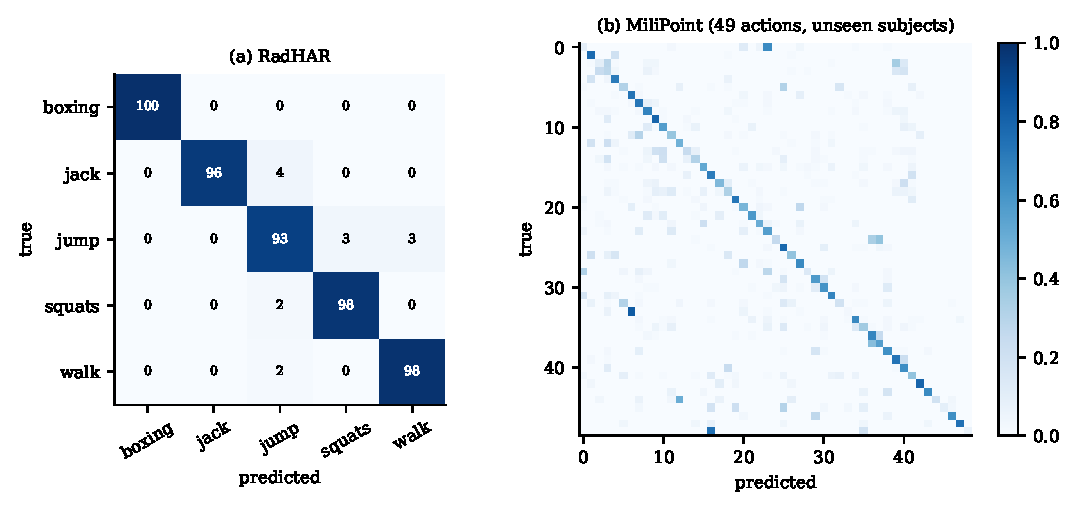
\includegraphics[width=\textwidth]{confusion.pdf}
\caption{Row-normalised confusion matrices of the proposed STPT-Lite+KD+robust (seed 0).}
\label{fig:confreport}
\end{figure}
\begin{table}[h]
\centering
\caption{Per-class test precision, recall and F1 (\%) of the proposed model (STPT-Lite+KD+robust) on RadHAR (mean over seeds).}
\label{tab:perclass}
\begin{tabular}{lrrrr}
\toprule
Class & Precision & Recall & F1 & Windows \\
\midrule
boxing & 99.86 & 99.91 & 99.88 & 714 \\
jumping jacks & 99.69 & 95.15 & 97.36 & 673 \\
jump & 91.01 & 94.41 & 92.66 & 734 \\
squats & 97.57 & 96.79 & 97.17 & 674 \\
walk & 96.83 & 97.79 & 97.31 & 770 \\
\bottomrule
\end{tabular}
\end{table}
On MiliPoint the per-action recall of the proposed model (mean over seeds) ranges from 6.4\% (action 33) to 83.9\% (action 9); 27 of 49 actions are recalled at $\geq$50\% and 6 below 20\%. The weakest actions are confused with kinematically similar ones (off-diagonal clusters in Fig.~\ref{fig:confreport}).

\section{Training and validation behaviour}
\begin{figure}[h]
\centering
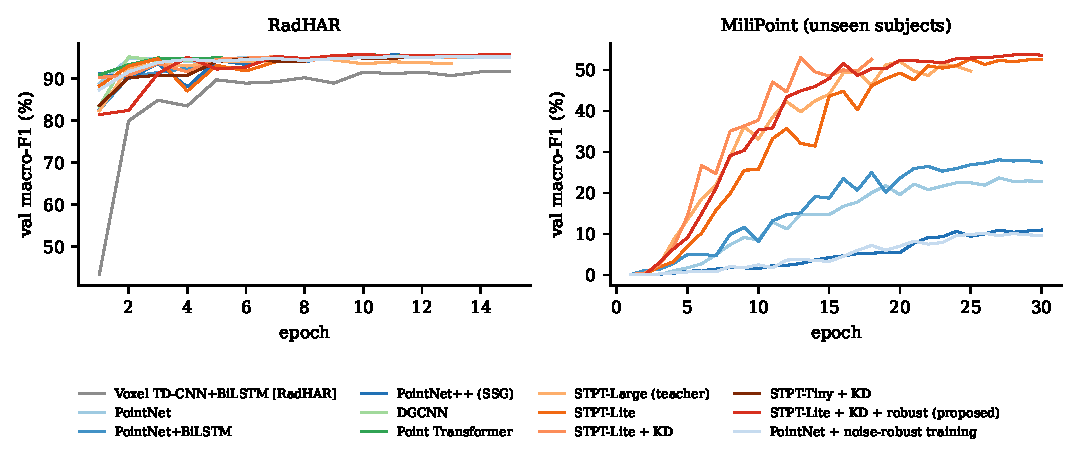
\includegraphics[width=\textwidth]{curves.pdf}
\caption{Validation macro-F1 per epoch (seed 0) for every model. RadHAR saturates within a few epochs; on MiliPoint the STPT models converge between epochs 15 and 30, while the PointNet family keeps a large gap.}
\label{fig:curvesreport}
\end{figure}
Training/validation loss, accuracy and learning rate for every epoch of every run
are stored in \texttt{results/runs/*/history.csv}. On RadHAR, 22 of 24 runs of the
cheaper models stopped early or peaked before the 15-epoch cap. On MiliPoint the
30-epoch cap was introduced after the first runs peaked at the 15-epoch cap
(Issue \#33). After the change, the STPT runs peaked between epochs 13 and 29.

\section{Ablation, protocol study and transfer}
\begin{table}[t]
\centering
\caption{Ablation of STPT-Lite (no distillation): test accuracy (\%), mean\,$\pm$\,std over seeds (variants: 2 on RadHAR, 2 on MiliPoint; full model: 3), change w.r.t.\ the full model trained with the same seeds in brackets; $^\dagger$ single run.}
\label{tab:ablation}
\setlength{\tabcolsep}{3pt}
\resizebox{\columnwidth}{!}{%
\begin{tabular}{lcc}
\toprule
Variant & RadHAR & MiliPoint (subj.) \\
\midrule
STPT-Lite (full, no KD) & 96.22\,$\pm$\,1.43 & 45.79\,$\pm$\,6.30 \\
\midrule
-- intra-segment attention (max+attentive pool only) & 96.90\,$\pm$\,0.18 (+0.93) & 42.87\,$\pm$\,3.03 (-6.52) \\
-- motion descriptor & 97.67\,$\pm$\,0.16 (+1.70) & 49.90\,$\pm$\,2.06 (+0.50) \\
-- temporal Transformer (mean over segments) & 96.70\,$\pm$\,0.61 (+0.73) & 37.54\,$\pm$\,6.62 (-11.85) \\
-- Doppler \& intensity ($xyz$ only) & 96.42\,$\pm$\,1.69 (+0.45) & -- \\
-- spatial gating & 97.62\,$\pm$\,0.40 (+1.64) & -- \\
-- all training augmentation & 96.68\,$\pm$\,0.54 (+0.70) & -- \\
-- coordinate jitter augmentation & 95.86\,$\pm$\,1.13 (-0.11) & -- \\
\bottomrule
\end{tabular}}
\end{table}
\textbf{MiliPoint (unseen people)} is the informative benchmark for the
architecture. Compared with the full model trained with the same two seeds
(49.4\% on average), removing the temporal Transformer (mean over segment
tokens instead) costs 11.9 points, and removing the intra-segment attention
(pooling only) costs 6.5 points. Both losses hold in each seed separately.
Fine-grained actions are therefore distinguished both by how the returns of a
short segment relate to each other and by how the segments evolve over the
window. The explicit motion descriptor brings no measurable gain (+0.5 points on
average, +2.8 and $-$1.8 in the two seeds): the attention layers apparently
recover centroid and displacement information from the point coordinates
themselves. We keep the descriptor because it costs only 2.5\,K parameters (2\% of the model), but
we do not claim it as a contribution to accuracy. \textbf{RadHAR} cannot rank
components. Every variant, including removing Doppler/intensity, gating or
augmentation, lies within about 1.7 points of the full model, inside its
seed spread ($\pm$1.4), because every model already exceeds 95\%. The
effect of the pre-processing is visible across models instead: with the same gating
and centring, all baselines exceed the published 90.47\%.


\begin{table}[t]
\centering
\caption{MiliPoint (49 actions) top-1 accuracy (\%) of the same models under three splits. Published numbers: 34.45 (PointNet++, \cite{cui2023milipoint}) and 98.25 (MAK-GCN, random 80/10/10, \cite{zakka2025makgcn}).}
\label{tab:protocol}
\setlength{\tabcolsep}{3pt}
\resizebox{\columnwidth}{!}{%
\begin{tabular}{lccc}
\toprule
Model & Subject-disjoint & Chronological & Random windows \\
 & (ours, primary) & (MiliPoint code) & (leaky) \\
\midrule
STPT-Lite & 45.79\,$\pm$\,6.30 & 58.38 (n=1) & 79.48 (n=1) \\
PointNet & 32.57\,$\pm$\,4.59 & 32.42 (n=1) & 44.44 (n=1) \\
\bottomrule
\end{tabular}}
\end{table}
\begin{table}[t]
\centering
\caption{Cross-dataset transfer (STPT-Lite, $xyz$ input): test accuracy (\%) when fine-tuning on a fraction of target training recordings/runs, from scratch vs.\ initialised from the model trained on the other dataset (mean\,$\pm$\,std, 3 seeds).}
\label{tab:transfer}
\setlength{\tabcolsep}{3pt}
\resizebox{\columnwidth}{!}{%
\begin{tabular}{llcc}
\toprule
Direction & Target data & Scratch & Pre-trained \\
\midrule
MiliPoint $\rightarrow$ RadHAR & 10\% & -- & -- \\
MiliPoint $\rightarrow$ RadHAR & 25\% & -- & -- \\
MiliPoint $\rightarrow$ RadHAR & 100\% & 95.23\,$\pm$\,0.00 & -- \\
\midrule
RadHAR $\rightarrow$ MiliPoint & 25\% & -- & -- \\
RadHAR $\rightarrow$ MiliPoint & 100\% & 45.79\,$\pm$\,6.30 & -- \\
\bottomrule
\end{tabular}}
\end{table}
\label{tab:transferreport}
Pre-training on MiliPoint helps most when little RadHAR data is available. With
10\% of the RadHAR training recordings it raises test accuracy from
\trrhxyzscratchfTen\% to \trrhxyzmpinitfTen\% (two seeds; +18 points, larger
than the seed spread). With 25\% the gain shrinks to about one point, inside the
seed spread, and with all training data the pre-trained and scratch models are
equivalent (\trrhxyzmpinitfFull\% vs.\ \trrhablxyz\%). Since the two datasets
differ in radar, frame rate, subjects, room and label set, this suggests that
the segment tokenizer learns largely sensor-independent motion features from MiliPoint's
49 actions, which are most valuable when target labels are scarce, as in a new
home with few annotated recordings. With all data, one pre-trained seed reached its best validation score after the
first epoch and was stopped early (93.8\%); we report it unchanged.


\section{Noise robustness}
\begin{figure}[h]
\centering
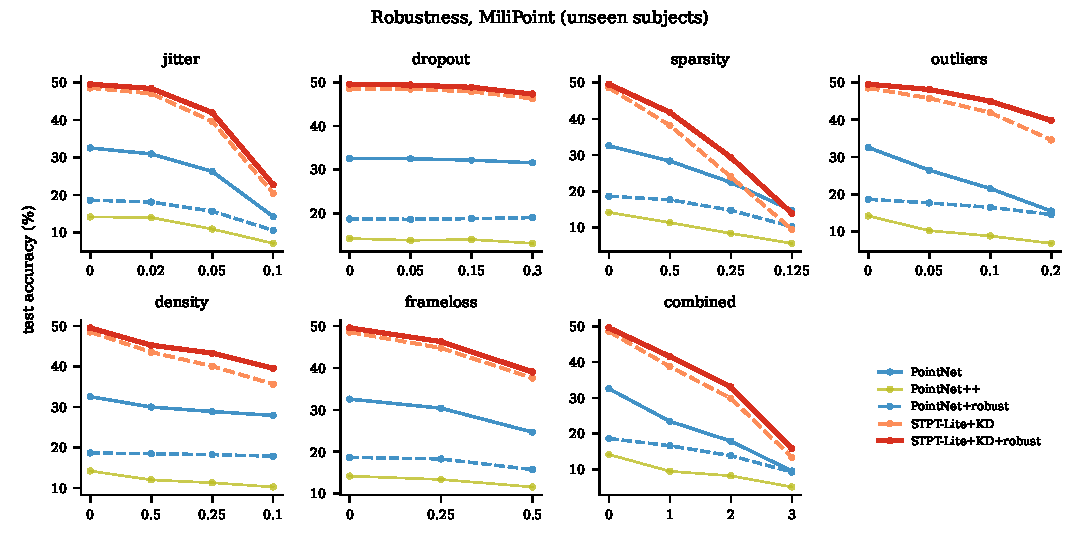
\includegraphics[width=\textwidth]{robustness_milipoint.pdf}
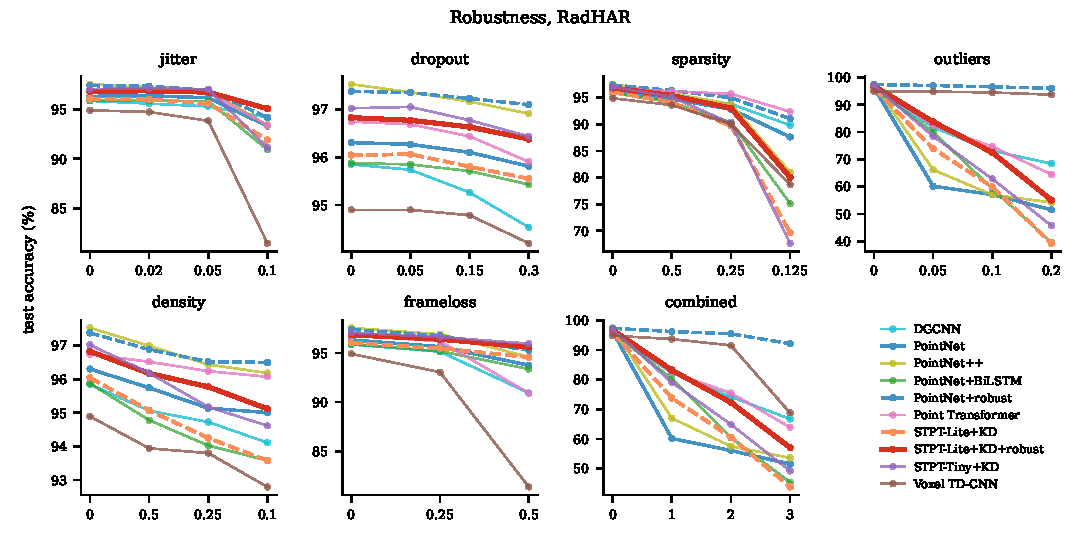
\includegraphics[width=\textwidth]{robustness_radhar.pdf}
\caption{Accuracy under controlled perturbations (identical perturbed test samples for every model). Top: MiliPoint; bottom: RadHAR.}
\label{fig:robreport}
\end{figure}
\begin{table}[h]
\centering
\caption{Robustness on MiliPoint (unseen subjects): test accuracy (\%) / prediction stability (\% of predictions unchanged w.r.t.\ clean), mean over seeds.}
\label{tab:robmilipoint}
\resizebox{\textwidth}{!}{%
\begin{tabular}{lccccc}
\toprule
Condition (level) & PointNet & PointNet+rob. & PointNet++ & STPT+KD & STPT+KD+rob. \\
\midrule
clean (0) & 32.6 / 100 & 18.7 / 100 & 14.2 / 100 & 48.5 / 100 & 49.6 / 100 \\
jitter (0.05) & 26.3 / 62 & 15.7 / 66 & 11.0 / 31 & 39.6 / 69 & 42.0 / 74 \\
dropout (0.3) & 31.6 / 73 & 19.0 / 69 & 13.1 / 53 & 46.3 / 77 & 47.3 / 80 \\
sparsity (0.25) & 22.5 / 35 & 14.8 / 29 & 8.4 / 20 & 24.0 / 29 & 29.4 / 38 \\
outliers (0.1) & 21.6 / 42 & 16.5 / 63 & 8.8 / 21 & 41.9 / 70 & 45.0 / 77 \\
density (0.25) & 28.9 / 57 & 18.2 / 50 & 11.3 / 38 & 40.1 / 58 & 43.3 / 64 \\
frameloss (0.5) & 24.7 / 44 & 15.8 / 38 & 11.6 / 30 & 37.6 / 59 & 39.0 / 61 \\
combined (2) & 17.9 / 30 & 13.8 / 36 & 8.2 / 14 & 29.9 / 44 & 33.0 / 51 \\
\bottomrule
\end{tabular}}
\end{table}
\begin{table}[h]
\centering
\caption{Robustness on RadHAR: test accuracy (\%) / prediction stability (\% of predictions unchanged w.r.t.\ clean), mean over seeds.}
\label{tab:robradhar}
\resizebox{\textwidth}{!}{%
\begin{tabular}{lccccc}
\toprule
Condition (level) & PointNet & PointNet+rob. & PointNet++ & STPT+KD & STPT+KD+rob. \\
\midrule
clean (0) & 96.3 / 100 & 97.4 / 100 & 97.5 / 100 & 96.0 / 100 & 96.8 / 100 \\
jitter (0.05) & 96.2 / 98 & 96.9 / 99 & 97.0 / 99 & 95.6 / 99 & 96.7 / 99 \\
dropout (0.3) & 95.8 / 99 & 97.1 / 99 & 96.9 / 99 & 95.5 / 99 & 96.4 / 99 \\
sparsity (0.25) & 92.8 / 96 & 95.0 / 97 & 93.8 / 96 & 89.7 / 92 & 93.0 / 95 \\
outliers (0.1) & 57.1 / 56 & 96.6 / 99 & 57.0 / 57 & 59.9 / 60 & 72.5 / 72 \\
density (0.25) & 95.1 / 98 & 96.5 / 99 & 96.4 / 98 & 94.2 / 98 & 95.8 / 98 \\
frameloss (0.5) & 93.7 / 96 & 95.2 / 97 & 94.6 / 96 & 94.6 / 97 & 95.6 / 98 \\
combined (2) & 56.0 / 55 & 95.5 / 98 & 57.5 / 57 & 60.5 / 61 & 72.3 / 72 \\
\bottomrule
\end{tabular}}
\end{table}

Fig.~\ref{fig:robust} reports test accuracy under seven perturbation types,
three severities each, applied with fixed seeds so that every model sees the
same perturbed windows. \textbf{MiliPoint (unseen people).} The proposed model
stays the most accurate under every condition except the most extreme
sparsity. Noise-robust training improves STPT-Lite+KD under all perturbations,
by 0.9--5.4 points (e.g.\ 20\% false detections: 34.6$\rightarrow$39.8\%; density
0.1: 35.6$\rightarrow$39.6\%), including jitter, which was not used in training
(22.8 vs.\ 20.5\% at $\sigma=10$\,cm). At 12.5\% of the returns kept (about one
point per frame), STPT-Lite (13.9\%) falls to the level of PointNet (14.7\%): with
almost no points per segment, intra-segment attention has nothing to attend to.
\textbf{RadHAR.} Dropout, density changes and jitter up to 5\,cm cost every
point-based model at most 2.5 points. Losing half of the segments costs DGCNN and
Point Transformer about five points but the proposed model only 1.2 points
(96.8$\rightarrow$95.6\%), which matches the even temporal attention in
Section~\ref{sec:xai}. Two conditions separate the
models. Under extreme sparsity, Point Transformer (92.4\%) and PointNet with
robust training (91.1\%) degrade least, the proposed model reaches 80.0\%, and
STPT-Lite+KD without robust training drops to 69.7\%. False detections are the
main weakness of the STPT family on RadHAR: at 20\% injected outliers the
proposed model keeps 55.1\% (39.3\% without robust training), whereas PointNet
with the same robust training keeps 96.0\% and the voxel CNN-LSTM 93.7\%.
A likely cause is that outliers corrupt the motion descriptor (centroid, mean Doppler) and receive
attention weight, while a max-pooled PointNet with robust training learns to
ignore isolated points and voxel occupancy dilutes them. Robust training
therefore helps, but it does not close this gap. A robust centroid (median) in
the motion descriptor and outlier-aware attention are the obvious next steps.


\section{Explainability}
\begin{figure}[h]
\centering
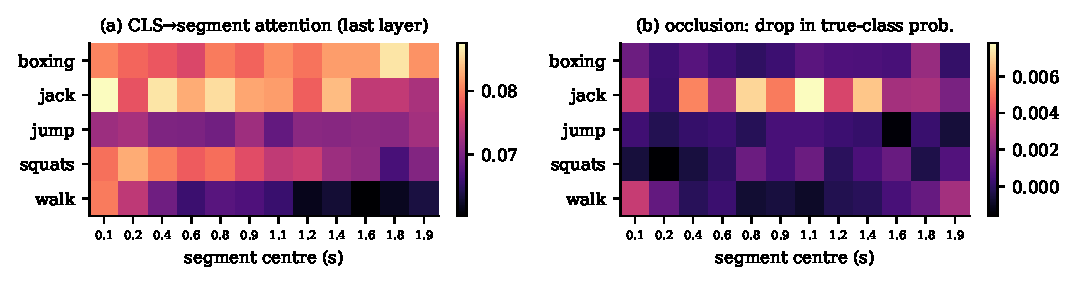
\includegraphics[width=\textwidth]{xai_temporal.pdf}
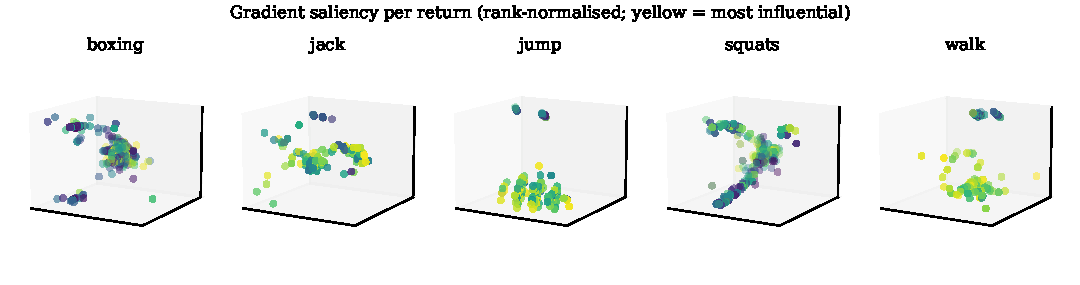
\includegraphics[width=\textwidth]{xai_saliency.pdf}
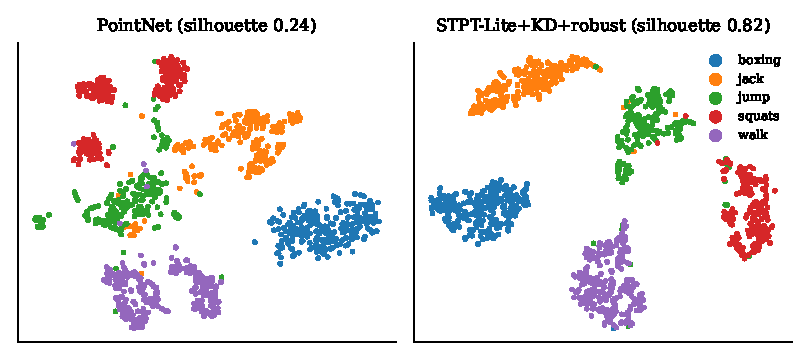
\includegraphics[width=0.75\textwidth]{tsne.pdf}
\caption{Temporal attention vs.\ occlusion importance, per-point gradient saliency, and t-SNE of embeddings (RadHAR test).}
\label{fig:xaireport}
\end{figure}
\textbf{Temporal attention and occlusion.} The [CLS] attention of the last
block is spread almost evenly over the twelve segments (0.07--0.09 per
segment, against 0.083 for uniform attention), with class-specific emphasis: the
middle of the window for jumping jacks, early segments for squats, and the
first segment for walking (Fig.~\ref{fig:xai}). Removing a single segment
(occlusion) lowers the true-class probability by less than one percentage point
on average. The model therefore integrates evidence over the whole window and
does not depend on any single 170-ms segment, which is consistent with its
tolerance to frame loss. Attention and occlusion importance agree only
moderately (Pearson $r=\xaiCorr$ over the class$\times$segment cells), so we
treat attention as a coarse indication and not as a faithful explanation.
\textbf{Point saliency.} Gradient saliency concentrates on the returns of the
moving limbs and torso and is low on isolated returns far from the body,
i.e.\ on the residual clutter that survives gating. \textbf{Embeddings.} In a
t-SNE of RadHAR test embeddings the classes form compact, well-separated
clusters (silhouette \silSTPTLiteKDrobust{} in the model's embedding space
versus \silPointNet{} for PointNet). \textbf{Errors.} The remaining RadHAR
errors are mostly windows predicted as \emph{jump} (precision 91\%), which
shares the strong vertical Doppler pattern of jumping jacks and squats. On
MiliPoint, errors concentrate in groups of kinematically similar actions.


\section{Computational efficiency}
\begin{figure}[h]
\centering
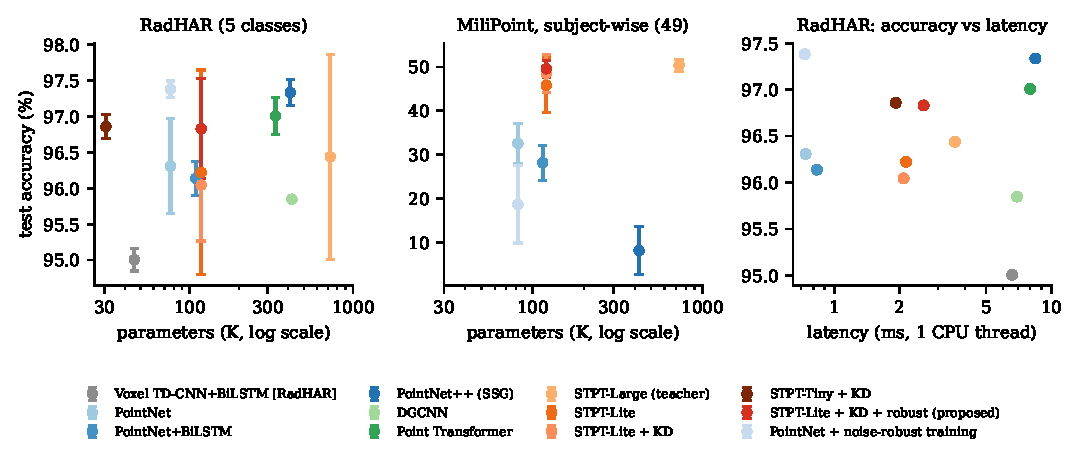
\includegraphics[width=\textwidth]{efficiency.pdf}
\caption{Accuracy vs.\ parameters and latency.}
\label{fig:effreport}
\end{figure}
STPT-Lite needs \oursMflops\,MFLOPs and \oursLat\,ms per 2-s window on one
CPU thread. It occupies \oursFpMB\,MB in FP32 and \oursIntMB\,MB with INT8
weights, and INT8 accuracy is unchanged (\rhOursIntAcc\% RadHAR,
\mpOursIntAcc\% MiliPoint).
